\chapter{Multi-class classification}

Multiclass classification is the problem of classifying instances into one of three or more classes. While many classification algorithms naturally permit the use of more than two classes, some are by nature binary algorithms; these can, however, be turned into multinomial classifiers by a variety of strategies.

Most of the real-world applications involve multiclass classification, for example: document classification, handwriting recognition, face recognition, sentiment analysis, autonomous vehicles, emotion recognition.

We will see that it's relatively easy to think of a binary classifier as a \emph{black box}, which can be reused for solving these more complex problems. This is a very useful abstraction, since it allows us to reuse knowledge, rather than having to build new learning models and algorithms from scratch.

Formally, given an input space \(X\) and a number of classes \(K\), an unknow distribution \(D\) over \(X \times [K]\), and a training set \(D'\) sampled from \(D\). The multiclass classification computes a function \(f\) minimizing \(\mathbb{E}_{(x,y)\sim D} [f(x) \neq y]\).

\section{Extension from binary}

This section discusses strategies of extending the existing binary classifiers to solve multi-class classification problems.

\subsubsection{\(k\)-nearest neighbours}
\(k\)-nearest neighbors is considered among the oldest non-parametric classification algorithms. To classify an unknown example, the distance from that example to every other training example is measured. The \(k\) smallest distances are identified, and the most represented class by these \(k\) nearest neighbours is considered the output class label. This kind of classification can by its nature handle multiclass classification problems, because it doesn't have any class constraint. 

\subsubsection{Decision trees}
Decision tree learning is a powerful classification technique. The tree tries to infer a split of the training data based on the values of the available features to produce a good generalization. The algorithm can naturally handle binary or multiclass classification problems. The leaf nodes can refer to any of the \(K\) classes concerned.

\subsubsection{Perceptron}
It is hard to separate three or more classes with just one line, so the perceptron algorithm need some changes to fit the multiclass classification problem.

Using a binary classifier as a black box, can reduce the task of multiclass classification to the binary case? There are multiple ways to decompose the multiclass prediction into multiple binary decisions. Two approaches are:
\begin{itemize}
    \item One-versus-all,
    \item All-versus-all.
\end{itemize}

\begin{figure}[t]
\begin{center}
    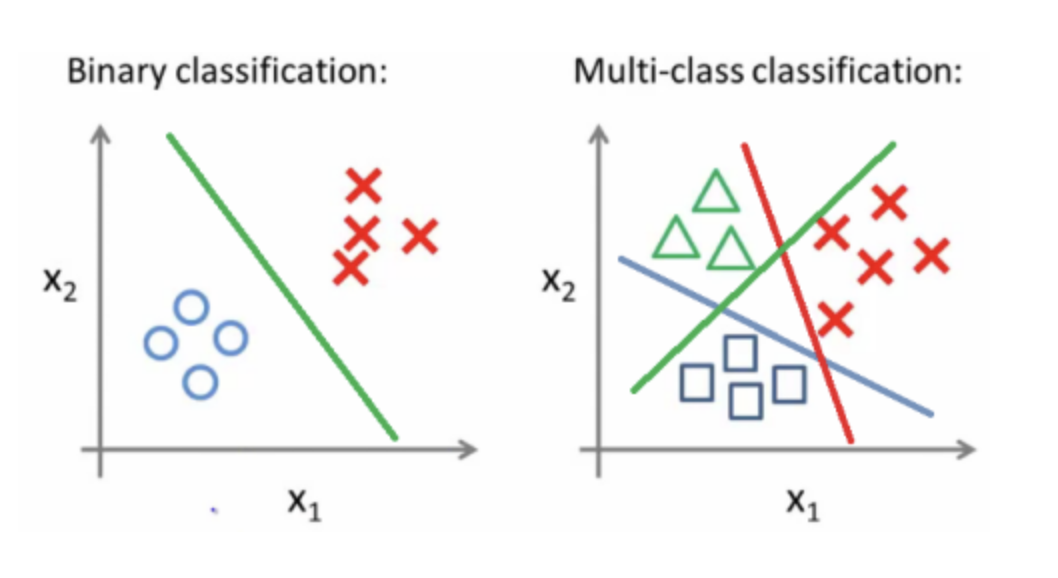
\includegraphics[width=.75\textwidth]{035}
	\vspace*{-35pt}
\end{center}
\caption{Binary classification vs Multiclass classification}
\label{fig:035}
\end{figure}

\section{One vs All}
A very common approach is the \textbf{one versus all} technique. To perform OVA, you train \(K\)-many binary classifiers \(f_1,...,f_K\). Each classifier sees all of the training data. Classifier \(f_i\) receives all examples labeled with class \(i\) as positives and all other examples as negatives.

At test time, whichever classifier predicts positive wins, with ties broken randomly.

\begin{algorithm}
    \caption{OneVersusAllTrain($D^\text{multiclass}$, $BinaryTrain$)}
    \label{alg:ovatrain}
\For{$i \gets 1,...,K$}{
	$D^\text{bin} \gets$ relabel $D^\text{multiclass}$ so class $i$ is positive, and class $\neg i$ is negative\;
	$f_i \gets \text{BinaryTrain}(D^\text{bin})$\;
}
\Return{$f_1,...,f_K$}
    \end{algorithm}

In the testing procedure, the prediction of the \(i\)th classifier is added to the overall score for class \(i\). Thus, if the prediction is positive, class \(i\) gets a vote; if the prediction is negative, every one else (implicitly) gets a vote.

	\begin{algorithm}
		\caption{OneVersusAllTest($f_1,...,f_K$, $x$)}
		\label{alg:ovatest}
		$score \gets \langle 0,0,...,0 \rangle$\;
	\For{$i \gets 1,...,K$}{
		$y \gets f_i(x)$\;
		$score_i \gets score_i + y$\;
	}
	\Return{$\text{argmax}_k\ score_k$}
		\end{algorithm}

OVA is quite natural and easy to implement. It also works very well in practice, so long as you do a god job choosing a good binary classification algorithm tuning its hyperparameters well.

Its weakness is that it can be somewhat brittle. Intuitively, it is not particularly robus to errors in the underlying classifiers. If one classifier makes a mistake, it is possible that the entire prediction is erroneous. In fact, it is entirely possible that \emph{none} of the \(K\) classifier predicts positive (which is actually the worst scenario)!

\section{All vs All}
To develop alternative approeaches, a useful way to think about turning multiclass classification problems into binary classification problems is to think of them like tournaments. You have \(K\) teams entering a tournament, but unfortunately the sport they are playing only allows two to compete at a time. 

One natural approach is to have every team compete against every other team. The team that wins the majority of its matches is declared the winner. This is the \textbf{all versus all} approach.

The most natural way to think about it is as training \(K \choose 2\) classifiers. Say \(f_{ij}\) for \(1 \leq i < j \leq K\) is the classifier that pits class \(i\) against class \(j\). This classifier receives all of the class \(i\) examples as positive and all of the class \(j\) examples as negative. When a test point arrives, it is run through all \(f_{ij}\) classifiers. Every time \(f_{ij}\) predicts positive, class \(i\) gets a point; otherwise, class \(j\) gets a point. After running all \(K \choose 2\) classifiers, the class with the most votes wins.

\begin{algorithm}
    \caption{AllVersusAllTrain($D^\text{multiclass}$, $BinaryTrain$)}
    \label{alg:avatrain}
	$f_{ij} \gets \emptyset, \forall 1 \leq i < j \leq K$\;
\For{$i \gets 1,...,K-1$}{
	$D^\text{pos} \gets$ all $x \in D^\text{multiclass}$ labeled $i$\;
	\For{$j \gets i+1,...,K$}{
		$D^\text{neg} \gets$ all $x \in D^\text{pos}$ labeled $j$\;
		$D^\text{bin} \gets \{(x, +1) : x \in D^\text{pos}\} \cup \{(x, -1) : x \in D^\text{neg}\}$\;
		$f_{ij} \gets BinaryTrain(D^\text{bin})$\;
	}
}
\Return{all $f_{ij}$}
    \end{algorithm}

	\begin{algorithm}
		\caption{AllVersusAllTest(all $f_{ij}$, $x$)}
		\label{alg:avatest}
		$score \gets \langle 0, 0, ..., 0 \rangle$\;
		\For{$i \gets 1,...,K-1$}{
			\For{$j \gets i+1,...,K$}{
			$y \gets f_{ij}(x)$\;
			$score_i \gets score_i + y$\;
			$score_j \gets score_j - y$\;
			}
		}
	\Return{$argmax_k\ score_k$}
		\end{algorithm}

\section{OVA vs AVA}
In terms of train time, AVA learns more classifiers, however, they are trained on much smaller data, and this tends to make it faster if the labels are equally balanced.

In terms of test time, AVA has more classifiers, so often is slower.

Furthermore, AVA trains on more balanced data sets, and test with more classifiers, therefore has more chances for errors.

If using a binary classifier, the most common thing to do is OVA. Otherwise, use a classifier that allows for multiple labels, for example decision trees and \(k\)-NN work reasonably well, but other more sophisticated methods work better.

\section{Evaluation}

Selecting the best metrics for evaluating the performance of a given classifier on a certain dataset is guided by a number of consideration including the class-balance and expected outcomes. One particular performance measure may evaluate a classifier from a single perspective and often fail to measure others. Consequently, there is no unified metric to measure the generalized performance of a classifier.

Two methods, \textbf{micro-averaging}, and \textbf{macro-averaging} are used to extract a single number for each of the precision, recall and other metrics across multiple classes.

\subsubsection{Micro-average}
In contrast, the micro-average calculates average metric from the aggregate contributions of all classes. Micro-average is used in unbalanced datasets as this method takes the frequency of each class into consideration. The micro average precision, recall, and accuracy scores are mathematically equivalent.
\begin{equation}
	\mu = \frac {\sum_{i=1}^N \text{score}_i} {\sum_{i=1}^N \text{score}_i + \text{frequency}_i}
\end{equation}

\subsubsection{Macro-average}
A macro-average calculates the metric autonomously for each class to calculate the average. This kind of average should be used only for balanced dataset, because otherwise it could be misleading.
\begin{equation}
	\mu = \frac {\sum_{i=1}^N \text{score}_i} N
\end{equation}

\begin{figure}[t]
	\begin{center}
		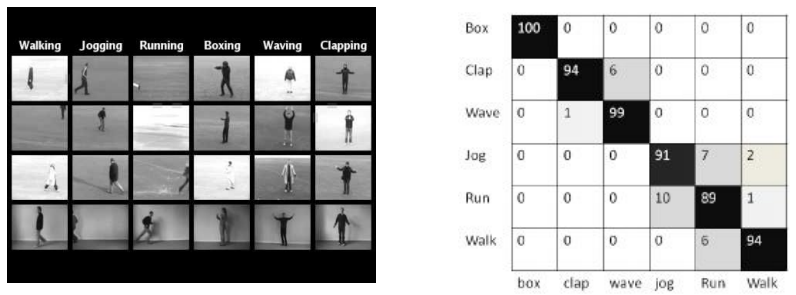
\includegraphics[width=0.75\textwidth]{036}
	\end{center}
	\caption{Confusion matrix example}
	\vspace*{-20pt}
	\label{fig:036}
\end{figure}
\subsection{Confusion matrix}
A confusion matrix shows the combination of the actual and predicted classes. Each row of the matrix represents the instances in a predicted class, while each column represents the instances in an actual class. It is a good measure of whether models can account for the overlap in class properties and understand which classes are most easily confused.

\newpage
\begin{exercise}[topsep=20pt,itemsep=10pt]
	\ex What is multiclass classification? 
	\ex What are the strategies to user binary classifiers for multiclass classification?
	\ex[!] Describe the OVA technique. Explain the training and the testing.
	\ex[!] Describe the AVA technique. Explain the training and the testing.
	\ex[!] How many classifiers are for OVA and how many for AVA?
	\ex[!] Compare OVA and AVA.
	\ex How do we evaluate a multiclass classification model?
	\ex What is a confusion matrix?
\end{exercise}